
\documentclass[a4paper]{article}
\usepackage[text={165mm,245mm}]{geometry}
\usepackage{graphicx}
\usepackage{subfigure}
\usepackage{ctex}
\usepackage{float} 
\usepackage{amsmath}
\usepackage{listings}
\usepackage{xcolor}
\definecolor{mygreen}{rgb}{0,0.6,0}  
\definecolor{mygray}{rgb}{0.5,0.5,0.5}  
\definecolor{mymauve}{rgb}{0.58,0,0.82}  
  
% RISC-V Assembler syntax and style for latex lstlisting package
% 
% These are risc-v commands as per our university (University Augsburg, Germany) guidelines.
%
% Author: Anton Lydike
%
% This code is in the public domain and free of licensing
\lstdefinelanguage[RISC-V]{Assembler}
{
  alsoletter={.}, % allow dots in keywords
  alsodigit={0x}, % hex numbers are numbers too!
  morekeywords=[1]{ % instructions
    lb, lh, lw, lbu, lhu,
    sb, sh, sw,
    sll, slli, srl, srli, sra, srai,
    add, addi, sub, lui, auipc,
    xor, xori, or, ori, and, andi,
    slt, slti, sltu, sltiu,
    beq, bne, blt, bge, bltu, bgeu,
    j, jr, jal, jalr, ret,
    scall, break, nop
  },
  morekeywords=[2]{ % sections of our code and other directives
    .align, .ascii, .asciiz, .byte, .data, .double, .extern,
    .float, .globl, .half, .kdata, .ktext, .set, .space, .text, .word
  },
  morekeywords=[3]{ % registers
    zero, ra, sp, gp, tp, s0, fp,
    t0, t1, t2, t3, t4, t5, t6,
    s1, s2, s3, s4, s5, s6, s7, s8, s9, s10, s11,
    a0, a1, a2, a3, a4, a5, a6, a7,
    ft0, ft1, ft2, ft3, ft4, ft5, ft6, ft7,
    fs0, fs1, fs2, fs3, fs4, fs5, fs6, fs7, fs8, fs9, fs10, fs11,
    fa0, fa1, fa2, fa3, fa4, fa5, fa6, fa7
  },
  morecomment=[l]{;},   % mark ; as line comment start
  morecomment=[l]{\#},  % as well as # (even though it is unconventional)
  morestring=[b]",      % mark " as string start/end
  morestring=[b]'       % also mark ' as string start/end
}
% language definition

\lstset{ %  
  backgroundcolor=\color{white},   % choose the background color; you must add \usepackage{color} or \usepackage{xcolor}  
  basicstyle=\footnotesize,        % the size of the fonts that are used for the code  
  breakatwhitespace=false,         % sets if automatic breaks should only happen at whitespace  
  breaklines=true,                 % sets automatic line breaking  
  captionpos=bl,                    % sets the caption-position to bottom  
  commentstyle=\color{mygreen},    % comment style  
  deletekeywords={...},            % if you want to delete keywords from the given language  
  escapeinside={\%*}{*)},          % if you want to add LaTeX within your code  
  extendedchars=true,              % lets you use non-ASCII characters; for 8-bits encodings only, does not work with UTF-8  
  frame=single,                    % adds a frame around the code  
  keepspaces=true,                 % keeps spaces in text, useful for keeping indentation of code (possibly needs columns=flexible)  
  keywordstyle=\color{blue},       % keyword style  
  %language=Bin,                 % the language of the code  
  morekeywords={*,...},            % if you want to add more keywords to the set  
  numbers=left,                    % where to put the line-numbers; possible values are (none, left, right)  
  numbersep=5pt,                   % how far the line-numbers are from the code  
  numberstyle=\tiny\color{mygray}, % the style that is used for the line-numbers  
  rulecolor=\color{black},         % if not set, the frame-color may be changed on line-breaks within not-black text (e.g. comments (green here))  
  showspaces=false,                % show spaces everywhere adding particular underscores; it overrides 'showstringspaces'  
  showstringspaces=false,          % underline spaces within strings only  
  showtabs=true,                  % show tabs within strings adding particular underscores  
  stepnumber=1,                    % the step between two line-numbers. If it's 1, each line will be numbered  
  stringstyle=\color{orange},     % string literal style  
  tabsize=2,                       % sets default tabsize to 2 spaces  
  %title=myPython.py                   % show the filename of files included with \lstinputlisting; also try caption instead of title  
}  
\title{\heiti 
CODH - 流水线CPU设计 \hspace{0.3cm}实验报告}
\author{院系: \kaishu\underline{}\hspace{1.5cm}姓名: \kaishu \underline{}\hspace{1.5cm}学号: \kaishu \underline{}\hspace{1.5cm}}
\begin{document}
\maketitle

\section{实验目的}
\begin{itemize}
    \item 理解流水线CPU的结构和工作原理
    \item 掌握流水线CPU的设计和调试方法,特别是流水线中的数据相关和控制相关的处理
    \item 熟练掌握数据通路和控制器的设计和描述方法
\end{itemize}

\section{实验环境}
\begin{itemize}
  \item macOS 13.0
  \item Rars1\_5.jar (Riscv Assembler and Runtime Simulator)
  \item Vivado 2019.3
  \item Nexys 4 DDR 开发板
\end{itemize}
\section{实验内容}
\subsection{流水线CPU数据通路的修改}
\begin{itemize}
    \item 添加级间寄存器存储不同阶段数据以及控制信号

  \end{itemize}

  \subsection{流水线CPU相关及其处理}
  \begin{itemize}
    \item 结构相关
    \item 数据相关
    \item 控制相关
  \end{itemize}
之后将指令和数据存储器用LabH3中的文件初始化后,与串行调试单元模块(SDU\_PL)整合,下载至FPGA中测试即可。

\section{逻辑设计 / 核心代码}
\subsection{流水线CPU数据通路的修改}
主要核心是四个级间寄存器的设计,它们是:
\begin{itemize}
    \item IF/ID 寄存器
    \item ID/EX 寄存器
    \item EX/MEM 寄存器
    \item MEM/WB 寄存器
  \end{itemize}

这些寄存器主要存储该阶段生成的需要传递到下一个阶段的数据,以及PC/IR值等。ID/EX寄存器需要存储EX阶段、MEM阶段、WB阶段的控制信号,
EX/MEM寄存器需要存储MEM阶段、WB阶段的控制信号,MEM/WB寄存器需要存储WB阶段的控制信号。

具体设计可以参照PPT中的数据通路图,部分寄存器可能需要额外存储某些信息,这里不再赘述。
\begin{figure}[H]
    \centering
    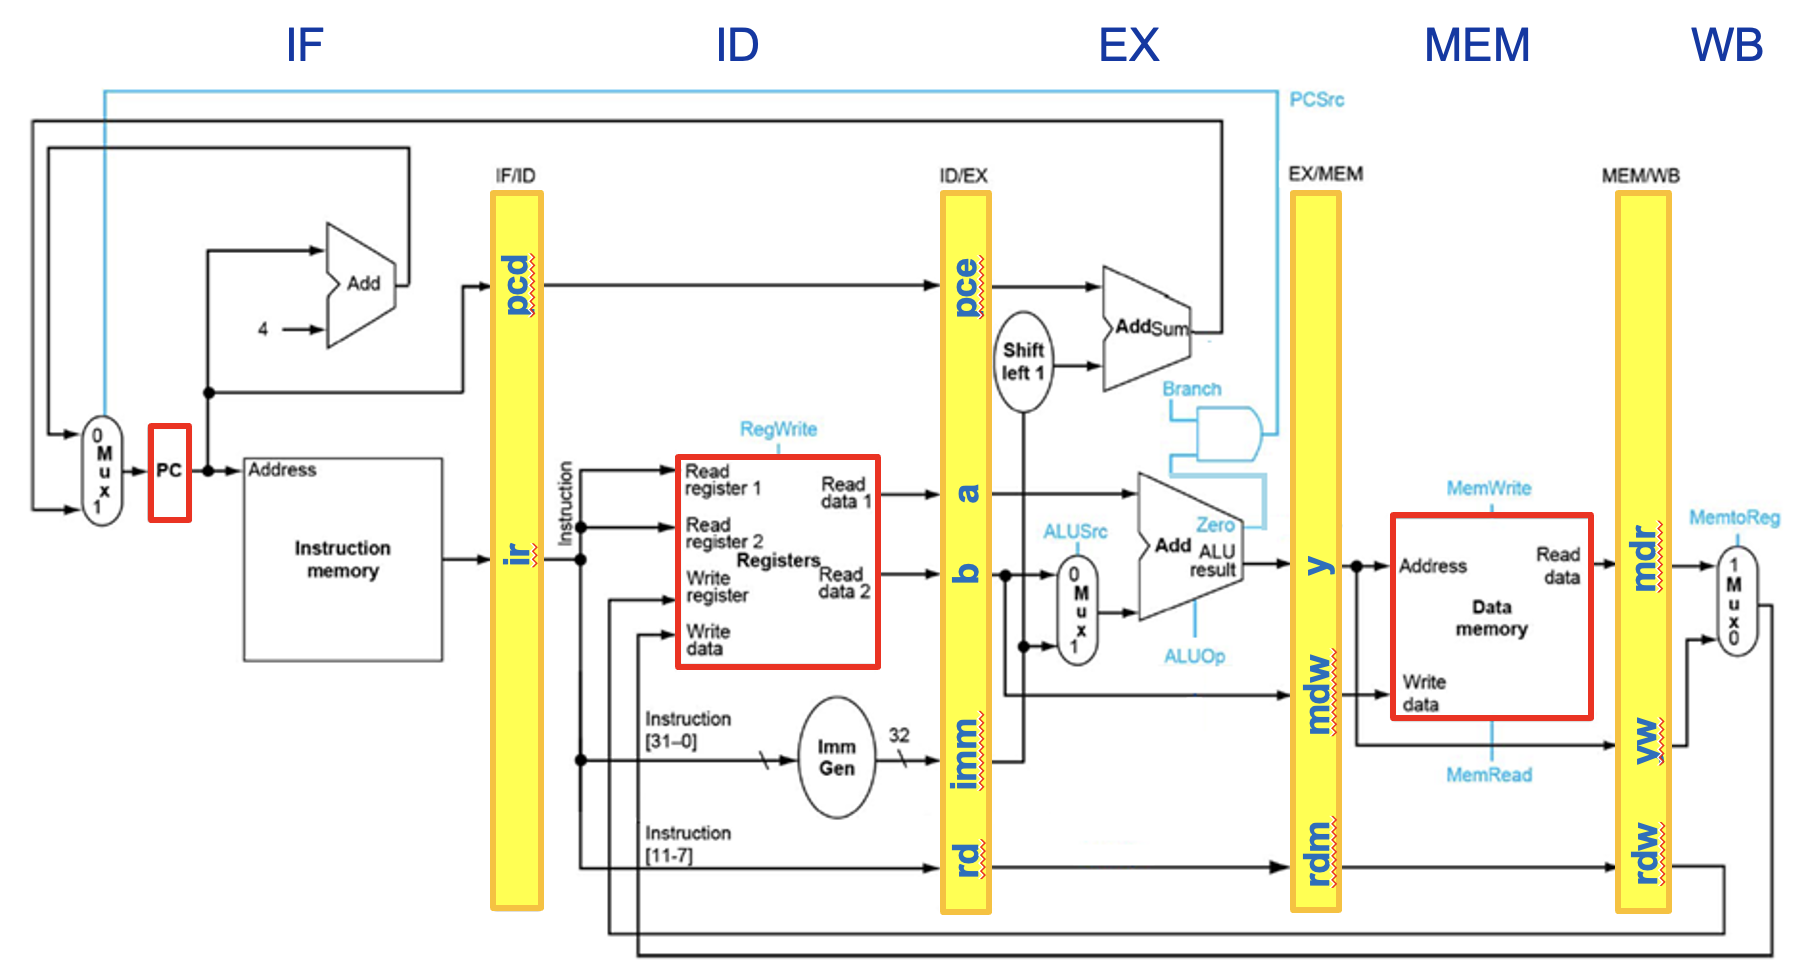
\includegraphics[width=0.9\textwidth]{1.png}
    \caption{CPU-fig}
    \label{fig:test1}
\end{figure}

下面列出这些寄存器的接口信息:
\begin{lstlisting}[language={verilog},title={cpu.v}] 
    IF_ID_reg IF_ID_reg_inst(
        .clk(clk), 
        .rstn(rstn),
        .stall(stall),
        .flush(flush),
        .pcd(IF_pc), 
        .ir(IF_ir), 
        ._pcd(ID_pc), 
        ._ir(ID_ir), 
        ._ra1(ID_rf_rs1), 
        ._ra2(ID_rf_rs2), 
        ._ire(ID_rf_rd)
    );

    ID_EX_reg ID_EX_reg_inst(
        //input - ID
        .clk(clk), 
        .rstn(rstn),
        .stall(stall),
        .flush(flush),
        .alu_src(ID_alu_src), 
        .alu_op(ID_alu_op),
        .pc_sel(ID_pc_sel),
        .mem_write(ID_mem_write),
        .reg_write(ID_reg_write),
        .reg_sel(ID_reg_sel),
        .pce(ID_pc),
        .ir(ID_ir),
        .a(ID_rf_rd1),
        .b(ID_rf_rd2),
        .rs1(ID_rf_rs1),
        .rs2(ID_rf_rs2),
        .imm(ID_imm),
        .ire(ID_rf_rd),
        //output - EX
        ._EX(EX_EX),
        ._mem_write(EX_mem_write),
        ._WB(EX_WB),
        ._pce(EX_pc),
        ._ir(EX_ir),
        ._a(EX_a),
        ._b(EX_b),
        ._imm(EX_imm),
        ._ire(EX_rf_rd),
        ._rs1(EX_rf_rs1),
        ._rs2(EX_rf_rs2)
    );

    EX_MEM_reg EX_MEM_reg_inst (
        //----INPUT----
        .clk(clk),
        .rstn(rstn),
        .mem_write(EX_mem_write),
        .WB(EX_WB),
        .imm(EX_imm),
        .pcm(EX_pc),
        .y(EX_alu_out),
        .mdw(EX_b),
        .irm(EX_rf_rd),
        .ir(EX_ir),
        .opcode(EX_opcode),
        //----OUTPUT----
        //control
        ._mem_write(MEM_mem_write),
        ._WB(MEM_WB),
        //data
        ._y(MEM_addr),
        ._pcm(MEM_pc),
        ._imm(MEM_imm),
        ._mdw(MEM_d),
        ._irm(MEM_rf_rd),
        ._ir(MEM_ir),
        ._opcode(MEM_opcode)
    );

    MEM_WB_reg MEM_WB_reg_inst(
        //----INPUT----
        .clk(clk),
        .rstn(rstn),
        .WB(MEM_WB),
        ._imm(MEM_imm),
        .pcw(MEM_pc),
        .mdr(MEM_dm_rd),
        .vw(MEM_addr),
        .irw(MEM_rf_rd),
        .ir(MEM_ir),
        .opcode(MEM_opcode),
        //----OUTPUT----
        //control
        ._reg_write(WB_reg_write),
        ._reg_sel(WB_reg_sel),
        //data
        ._mdr(WB_data),
        ._vw(WB_vw),
        ._irw(WB_rf_rd),
        ._pcw(WB_pc),
        .__imm(WB_imm),
        ._ir(WB_ir),
        ._opcode(WB_opcode)
    );

\end{lstlisting}

在ID阶段产生控制信号后,通过寄存器传递至后面的阶段即可利用,至此便得到了在非特殊情况下可正常运作的流水线CPU


\subsection{流水线CPU相关及其处理}
具体有三种相关需要特殊考虑,否则由于流水线CPU的特性不能正常运行。
\subsubsection{结构相关}
多条指令可能会同时访问一个存储。而一个存储器同一时钟周期只能写一次,考虑到这一点,我们采用哈佛结构,将指令存储器和数据存储器区分开来,这样便解决了端口冲突的问题。

另外有可能在WB阶段末尾需要写回的寄存器在下一个时钟周期的ID阶段就要读取。由于是时钟上升沿才进行写回,所以需要将寄存器改为写优先的读方式来解决这一问题,如下:
\begin{lstlisting}[language={verilog},title={cpu.v}] 
    assign rd1 = (ra1 == wa && we && wa != 0) ? wd : rf[ra1];  
\end{lstlisting}

\subsubsection{数据相关}
这一般出现在次条指令需要用到前面指令的运算结果时,分为两种情况:
\begin{enumerate}
    \item 前一条指令是LOAD指令之外的指令。次条指令段最晚在EX阶段需要将alu\_in的值替换为前一条指令的运算结果,此时上一条指令(或者更早)恰好执行到了MEM/WB阶段,可以将此阶段寄存器读出的
    运算结果forward至下一条指令的EX阶段输入即可。
    \item 前一条指令是LOAD指令,则LOAD的结果至少在MEM阶段结束(WB阶段开始时)时才可用forward到上一条指令的EX阶段。因此需要阻止紧随Load已进入流水线的指令流动(Stall),向后续流水段插入空操作(Bubble)。
\end{enumerate}
\begin{lstlisting}[language={verilog},title={cpu.v}] 
    forward forward_inst(
        .EX_rs1(EX_rf_rs1),
        .EX_rs2(EX_rf_rs2),
        .MEM_rd(MEM_rf_rd),
        .WB_rd(WB_rf_rd),
        .MEM_reg_write(MEM_WB[3]),
        .WB_reg_write(WB_reg_write),
        .MEM_reg_sel(MEM_WB[2:0]),
        .WB_reg_sel(WB_reg_sel),
        .EX_a(EX_a),
        .EX_b(EX_b),
        .MEM_alu_out(MEM_addr),
        .WB_rf_wd(WB_rf_wd),
        .alu_in1(a_forward),
        .alu_in2(b_forward),
        .MEM_pc(MEM_pc),
        .MEM_dm_rd(MEM_dm_rd),
        .MEM_imm(MEM_imm)
    );
\end{lstlisting}



具体的实现方式是编写forward模块,如果识别到EX阶段所读的寄存器地址恰好是MEM阶段/WB阶段的目标寄存器地址,则用MEM阶段/WB阶段的运算结果提前替换EX阶段的alu\_in值,否则不做任何操作。

而对于紧随LOAD指令的指令,需要让其暂停一个时钟周期,这里采用编写stall模块(实际把stall和后文的flush模块合并在一起了),如果识别到EX阶段所读的寄存器地址恰好是上一条指令MEM阶段的目标寄存器地址,且上一条指令恰好为LOAD,
则将stall信号置为1,否则为0。级间寄存器若识别到stall信号为1,则不在时钟上升沿写入数据,而是将数据保持不变,这样便实现了暂停一个时钟周期的功能。

\subsubsection{控制相关}
这方面的问题主要是由于控制相关指令决定跳转与否至少需要到EX阶段才能确定,而此时ID阶段已经读取了下一条指令。因此需要根据branch信号以及EX阶段的opcode来判断当前指令是否会产生跳转,
若是,则当前IF/ID阶段按顺序读取的两条指令都是错误的(应该改为正确的跳转后的指令),因此置flush信号为1。级间寄存器若识别到flush信号为1,则不在时钟上升沿写入数据,而是将数据清零,这样便实现了清空IF/ID寄存器,ID/EX寄存器的功能,
使得错误的指令不会进入流水线。
\begin{lstlisting}[language={verilog},title={cpu.v}] 
    stall_flush stall_flush_inst(
        .branch(branch),
        .opcode(EX_opcode),
        .ire(EX_rf_rd),
        .rf_rs1(ID_rf_rs1),
        .rf_rs2(ID_rf_rs2),
        .stall(stall),
        .flush(flush)
    );
\end{lstlisting}


\begin{lstlisting}[language={verilog},title={stall\_flush.v}] 
    always@(*) begin
        if ((opcode == I_LOAD) && ((ire == rf_rs1) || (ire == rf_rs2)))
            stall = 1;
        else
            stall = 0;

        if (branch || (opcode == J_JAL) || (opcode == I_JALR)) begin
            flush = 1;
        end
        else begin
            flush = 0;
        end
    end
\end{lstlisting}


烧录后测试程序以及排序程序的正确性已经由助教检查完成,流水线CPU设计任务至此完成。

\subsubsection{结果分析}
RTL电路:
\begin{figure}[H]
    \centering
    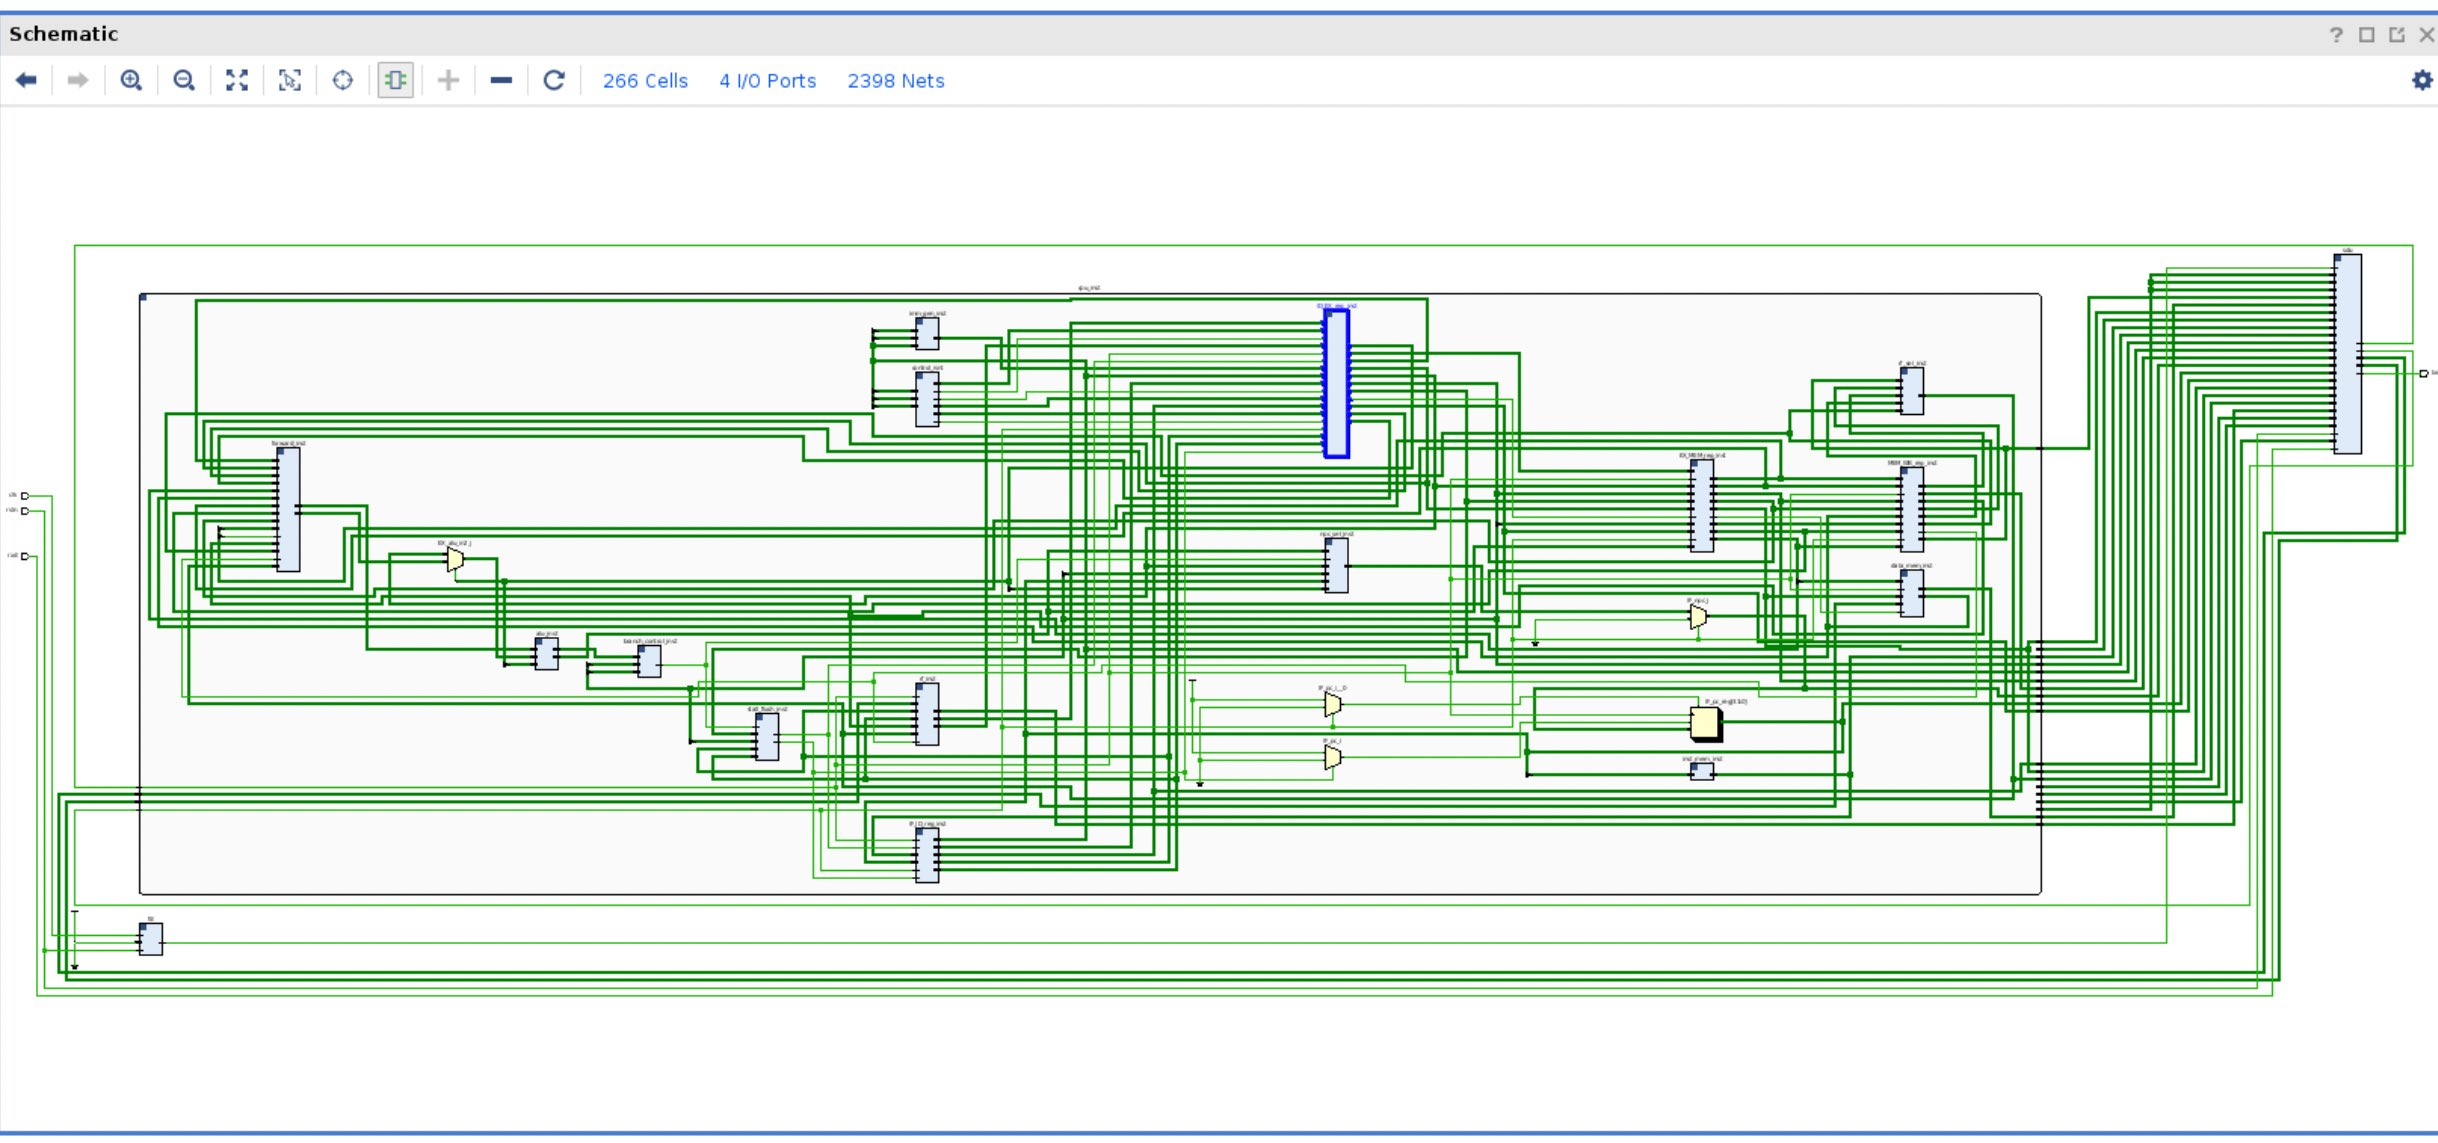
\includegraphics[width=0.9\textwidth]{2.jpg}
    \caption{RTL}
    \label{fig:test1}
\end{figure}

电路资源使用情况:
\begin{figure}[H]
    \centering
    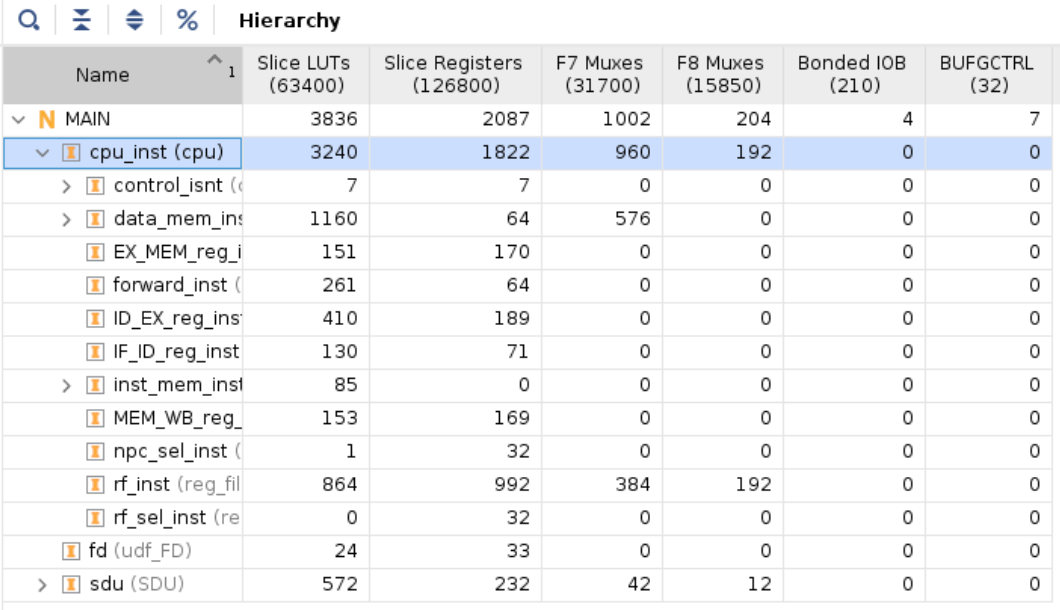
\includegraphics[width=0.9\textwidth]{4.png}
    \caption{UTL1}
    \label{fig:test1}
\end{figure}


电路性能:
\begin{figure}[H]
    \centering
    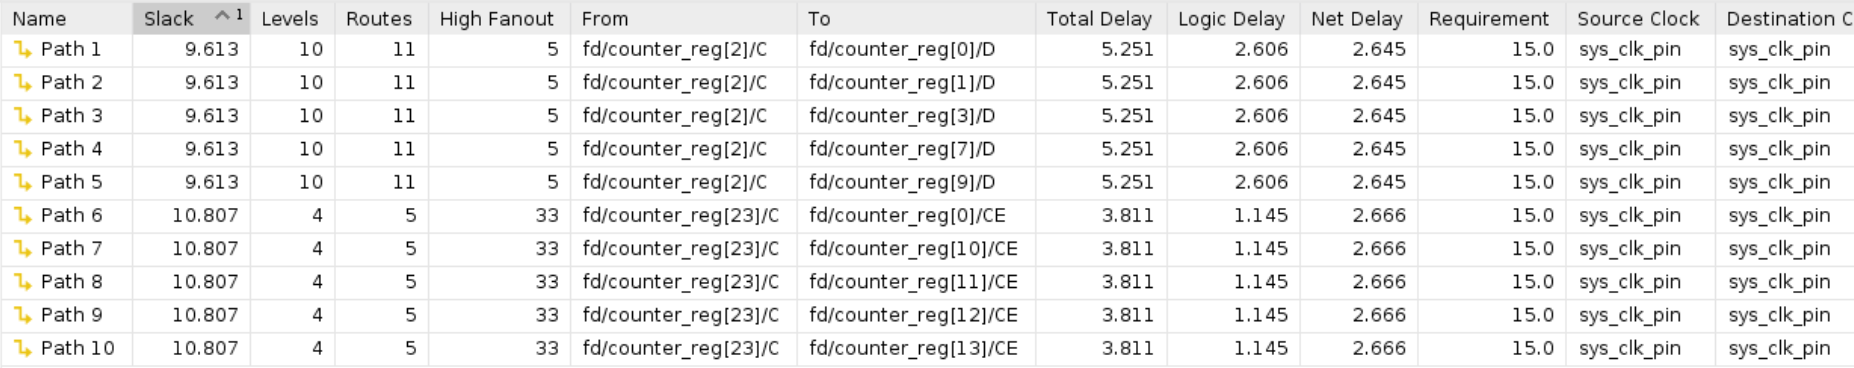
\includegraphics[width=0.9\textwidth]{3.png}
    \caption{TIMING}
    \label{fig:test1}
\end{figure}

\section {实验总结}
\begin{enumerate}
  \item 通过本次实验,我学习到了如何依据需求设计流水线CPU的数据通路,也就是如何修改单周期CPU的数据通路
  \item 通过本次实验,我理解了CPU各阶段之间的数据依赖关系以及控制信号关系
  \item 通过本次实验,我了解了流水线CPU相较于但周期CPU可能出现的不稳定因素,例如数据相关、控制相关等,以及如何通过设置相关模块机制(forward、flush、stall)解决这些问题
  \item 通过本次实验,我充分体会到了命名清晰的重要性,花费一定时间修改命名也可以让后续开发更加顺利
  \item 最重要的是,在本次试验中,所有编写调试编译生成操作全是在M1芯片平台上进行的。经过漫长的两个月后,终于可以在M1芯片上编译运行代码调试开发板了,这是一个值得庆祝的事情。
\end{enumerate}
\section {意见/建议}
无,这个实验设计很完美。希望实验文档再详细一些就好了
\end{document}